\documentclass[12pt]{article}
\usepackage[margin=1in]{geometry}
\usepackage[all]{xy}
\usepackage{multicol}

\usepackage{amsmath,amsthm,amssymb,color,latexsym}
\usepackage{geometry}        
\geometry{letterpaper}    
\usepackage{graphicx}
\usepackage[shortlabels]{enumitem}
\usepackage[dvipsnames]{xcolor}
\usepackage[linktoc=all]{hyperref}

\newtheorem{thm}{Theorem}
\newtheorem{defn}{Definition}
\newtheorem{cor}{Corollary}
\newtheorem{prop}{Proposition}
\newtheorem{lem}{Lemma}
\newtheorem{rmk}{Remark}

\numberwithin{thm}{section}
\numberwithin{defn}{section}
\numberwithin{prop}{section}
\numberwithin{rmk}{section}


\newcommand{\RR}{\mathbb{R}}
\newcommand{\NN}{\mathbb{N}}
\newcommand{\QQ}{\mathbb{Q}}
\newcommand{\FF}{\mathbb{F}}
\newcommand{\ZZ}{\mathbb{Z}}
\newcommand{\CC}{\mathbb{C}}
\newcommand{\ol}{\overline}
\newcommand{\AutG}{\text{Aut($G$)}}
\newcommand{\vp}{\vec{v}_p}
\newcommand{\f}{f:S\subset\CC\to\CC}
\newcommand{\q}[1]{\textbf{#1)}}
\newcommand{\ex}{Example }
\newcommand{\exs}{Examples }
\newcommand{\Hom}[2]{\text{Hom}(#1,#2)}
\definecolor{light-gray}{gray}{0.75}
\newcommand{\bra}[1]{\langle #1 \vert}
\newcommand{\ket}[1]{\vert #1 \rangle}
\newcommand{\braket}[2]{\langle #1\vert #2 \rangle}

\title{Introduction to Quantum Interactive Proof Systems}
\author{Liam Salt\\APMA 990}
\begin{document}
	\maketitle
	
	\begin{abstract}
		In this paper, we introduce quantum interactive proof systems, demonstrate their advantages over classical systems, and showcase an application by using them to prove certain properties of finite groups. We begin by introducing interactive proof systems as defined classically before extending to the quantum case, whereby we show that any language in PSPACE has a $2$-round quantum interactive proof system, which is strictly more powerful than the classical case. Then, we show an application to group theory wherein succinct (polynomial length) proofs for group non-membership are possible with a quantum proof system, which is impossible classically. Construction of efficient proofs for group non-membership also allows us to approach other group theoretical problems, such as finding the maximal normal subgroup and finding whether an integer divides the order of a group.
	\end{abstract}
	\section{Introduction}
	
	\subsection{Some Computer Science Background}
	
	Before we can begin to define a quantum proof system, we first must introduce some classical computing formalism and terminology. In classical computing, an \textit{interactive proof system} is a Turing machine that encapsulates the mathematical idea of a proof. It models a proof as a sequence of communications between two actors: a potentially dishonest \textit{prover}, and a skeptical, honest \textit{verifier}. Through various \textit{rounds} of communication, the prover attempts to convince the verifier to accept their proof. The typical convention (used in this paper) is to assume the verifier is constrained to be a deterministic polynomial-time Turing machine, whereas we make no constraints to the computational power of the prover. Additionally, an interactive proof system is assumed to satisfy the following two properties:
	\begin{enumerate}[label=(\roman*)]
		\item An interactive proof system is said to be \underline{complete} or to satisfy completeness if for any true statement, the prover can always convince the verifier of its validity.
		\item An interactive proof system is said to be \underline{sound} if for any false statement, the prover can only with negligible probability convince the verifier of its validity.
	\end{enumerate}

	\begin{rmk} Often, many of these conditions are loosened in various ways, e.g. the prover only needing to convince the verifier up to some probability.\end{rmk}
	
	Now we can more formally define a (deterministic) interactive proof system.\\
	
	\begin{defn}
	We say that a formal language $L$ has a\underline{ deterministic $k$-round interactive proof system} with error probability $\varepsilon$ with prover verifier pair $(P,V)$ if all of the following:
	\begin{enumerate}[label=(\roman*)]
		\item $(P,V)$ either accepts or rejects any input after $k$ rounds.
		\item $\forall x\in L, (P,V)$ accepts $x$ with probability 1.
		\item $\forall x\notin L, (P,V)$ accepts $x$ with probability $\varepsilon$.
	\end{enumerate}
	Any such languages are said to lie in the class \textbf{dIP}.
	\end{defn}
	Given this definition, a familiar, degenerate example is to show that any language in \textbf{NP} has a $1-$round interactive proof system with error probability $0$. We recall that one definition of \textbf{NP} is as the set of decision problems whose positive answers can be verified in polynomial time by a deterministic Turing machine. Accordingly, if a problem is in \textbf{NP}, then by definition on input our prover can produce a polynomial-sized certificate, which can be verified in polynomial-time exactly when the input is in the language. In fact, \textbf{dIP} is exactly equal to \textbf{NP}, that is we can capture the full power of deterministic interactive proof systems exactly with the class \textbf{NP}.\\
	
	We can generalize the above definition by allowing the verifier to also have access to a random number generator, with which it may generate and make use of uniformly random bits in each round. The addition of the verifier's access to randomness brings us to the full definition of an interactive proof system. The complexity class of all languages that have interactive proof systems is termed \textbf{IP}, and it can be shown that \textbf{IP}$=$\textbf{PSPACE} (\hyperref[kit00]{[Kit00]}). In other words, problems which can be accepted by an interactive proof system are exactly those problems which require only polynomial-sized space (memory) to answer. 
	\subsection{Arthur-Merlin Protocol}
	Related to \textbf{IP}, another class which will become important in the quantum case is \textbf{MA}, which stands for Merlin-Arthur (of King Arthur fame), and is comprised of languages which have a particular type of interactive proof system known as a Merlin-Arthur protocol. This class was originally described in \hyperref[bab]{[Bab85]} and \hyperref[gol89]{[Gol89]}.
	
	\begin{defn}
		A language $L$ is said to have a \underline{Merlin-Arthur protocol} with prover-verifier pair (Merlin, Arthur) or that $L$ is in the class \textbf{MA} if:
		\begin{enumerate}[label=(\roman*)]
			\item Arthur has access to random bits $y\in B_m$, which are known to Merlin.
			\item If $x\in L$, then there exists $z\in B_n$ such that $P(\text{Arthur accepts }x|y,z)\geq \frac{2}{3}$.
			\item If $x\notin L$, then for any $z\in B_n$ such that $P(\text{Arthur accepts }x|y,z)\leq\frac{1}{3}$. 
			\item $n,m$ are both polynomial-length.
		\end{enumerate}
	
	
	\end{defn}
	 For clarity, in the above definition $z$ is the polynomial-sized proof certificate provided by Merlin, and whether Arthur accepts Merlin's proof depends on both the string sent by Merlin and the random string produced by Arthur.\\
	
	The probability conditions given above are quite flexible. Given a language with a Merlin-Arthur protocol, it can be shown that we can induce a new Arthur-Merlin pair for that language that achieves perfect completeness, and soundness with error probability at most $\frac{1}{2}$ (\hyperref[wat00]{[Wat00]}]).\\
	
	Moving forward, it will be important to see how \textbf{MA} relates to other complexity classes:
	\begin{prop}\textbf{MA} contains both \textbf{NP}$=$\textbf{dIP} and \textbf{BPP}. \end{prop}
	\begin{proof}The second containment is easy to see given the definition of \textbf{BPP}, as Arthur has access to random bits and a polynomial-time Turing machine (with acceptance prob $\frac{2}{3}$ as required in \textbf{BPP}); therefore, Arthur need not send anything to Merlin, as he is capable of solving any problem in \textbf{BPP} himself.\\Similarly for \textbf{NP}, Merlin can solve the problem then send Arthur the proof certificate which he can verify deterministically, i.e. without needing his random bits. \end{proof}
	
    \section{Quantum Interactive Proof Systems}
    Now that we have seen the definition of interactive proof systems in the classical case, we can discuss what happens if we allow the Turing machines access to quantum computations. It has been observed that allowing access to quantum computation lends itself to significant speed-up in many classical problems (integer factorization, computing discrete logarithms, efficient unstructured search, etc.), so it makes sense to ask whether any of the above definitions in Section 1 are significantly affected by access to quantum circuits. It turns out that here, as in the case of Deutsch-Jozsa, we see that the principal speedup comes in the form of query complexity, or in our case, the number of rounds required in our proofs.
   
    \begin{rmk}The Turing machine model is sufficient, but for the remainder of this paper we will use the equivalent circuit model of quantum computation. \end{rmk}
    
    Specifically, a quantum interactive proof system is one where the verifier has access to quantum circuits which can solve problems in \textbf{BQP}, while the prover is still unrestricted (within the boundaries of quantum mechanics). The convention is for the messages exchanged between prover and verifier to be encoded as quantum states in the usual $n-$qubit $Z$-basis, however this is not strictly required. Some relevant terminology is that we call the class of all languages that have quantum interactive proof systems Quantum \textbf{IP} or \textbf{QIP}.
    \begin{defn}
    	A language $L$ is said to have a quantum interactive proof system with error probability $\varepsilon$, or to be in \textbf{QIP}, if for any input $x$:
    	\begin{enumerate}
    		\item The verifier accepts or rejects $x$ using a quantum circuit solving problems in \textbf{BQP}.
    		\item If $x\in L$, then after polynomial-many rounds of communication, the verifier accepts $x$ with probability $1$.
    		\item If $x\notin L$, then regardless of the actions of the prover, the verifier accepts $x$ with probability  at most $\varepsilon$.
    	\end{enumerate}
    \end{defn}

	We can see that this definition for \textbf{QIP} looks quite similar to the classical definition of \textbf{IP}, which we discuss more in the next section. In its current state \textbf{QIP} is actually only as powerful as \textbf{IP}, and in fact, \textbf{QIP}=\textbf{IP} = \textbf{PSPACE}, which is shown in \hyperref[wat09]{[Wat09]}. 
	\subsection{Relationship between QIP and PSPACE}
	Despite the simplicity of the claim at the end of the previous section, we can say a bit more about the relationship between \textbf{QIP} and \textbf{PSPACE}. Namely, we can put a very nice bound on the number of queries required in a quantum interactive proof system to determine any language in \textbf{PSPACE}. In fact, we can prove that \textbf{PSPACE} $\subseteq$ \textbf{QIP[2]}, the class of languages with $2$-round quantum interactive proof systems, a much tighter bound than what was claimed in the previous section. Importantly, this also shows that in the constant round case, \textbf{IP[k]} is strictly outperformed by \textbf{QIP[2]}, demonstrating the power of moving to quantum computations. We therefore introduce the first theorem, which is the principal subject of \hyperref[wat99]{[Wat99]}:
	
	\begin{thm}
		\label{thm1}
		Every language in \textbf{PSPACE} has a $2$-round quantum interactive proof system with exponentially small error probability. 
	\end{thm}
	
	
	To prove the above theorem, we need to show that any language in \textbf{PSPACE} has a $2$-round quantum proof system, but it will be sufficient to prove the theorem for a language which is \textbf{PSPACE}-complete. In particular, we show the theorem for the language of\textit{ true quantified boolean formulas (QBF)}, that is the language of true expressions $Q=Q_1x_1\cdots Q_nx_nf(x_1,\dots,x_n)$, where $Q_i$ is a universal or existential quantifier $(\forall,\exists)$, $x_i$ are boolean valued variables, and $f$ is a boolean formula $B_n\to B$ consisting of operations $\wedge,\vee,$ and $\neg$ on the variables $x_1,\dots,x_n$. \\
	
	There is a classical protocol outlining an interactive proof system for the QBF problem \hyperref[she92]{[She92]}, but this is general takes $N={{n+1}\choose{2}}+n$ rounds of communication, i.e. quadratic rounds with respect to number of variables. A full description of this classical protocol is not shown in this paper, but it is outlined in \hyperref[wat99]{[Wat99]}:
	
	\noindent A general outline of the algorithm for a formula $Q=Q_1x_1\cdots Q_nx_nf(x_1,\dots,x_n)$ of length $d$ with $n$ variables is:
	 \begin{enumerate}
	 	\item The verifier sends the prover a uniformly random element $r_1$ of a chosen finite field, and gets a corresponding function $f_1$ in response from the prover.
	 	\item They continue this exchange $N$ times, with each response polynomial $f_i$ being at most $\deg d$ and  depending only on the previously received random elements $r_1,\dots,r_{i}$. 
	 	\item After receving  the final $f_N$, the verifier inputs all of the data they have collected into a single predicate (evaluable in polynomial-time): $E(Q,r_1,\dots,r_N,f_1,\dots,f_N)$, which is defined in \hyperref[she92]{[She92]}.
	 	\item The verifier accepts if and only if $E(Q,r_1,\dots,r_N,f_1,\dots,f_N)$ evaluates to true.
	 \end{enumerate}
	 	
	After some analysis, this serves to prove that in the classical case, \textbf{IP} = \textbf{PSPACE}, and we therefore have already that \textbf{PSPACE} $\subseteq$ \textbf{QIP}, as we can simulate the classical circuit in the quantum case. Thus, it remains to show that allowing our system access to quantum circuits helps to reduce the number of rounds.\\
	
	Now, we outline a proof of \hyperref[thm1]{Theorem 2.1} by showing existence of a correct $2-$round quantum protocol for the language of true quantified boolean formulas.
	
	\begin{proof}
	We construct a quantum circuit which consists of three 2D arrays of quantum registers: $\textbf{R}=\{\textbf{R}\}_{i,j},\textbf{S}=\{\textbf{S}\}_{i,j},$ and $\textbf{F}=\{\textbf{F}\}_{i,j}$, for $1\leq i\leq m$ and $1\leq j\leq N$, where $N={{n+1}\choose{2}}+n$ as above, and $m=q(n)$ for some polynomial $q$. There are $m\cdot N$ many registers found in the collections $\textbf{R}$ and $\textbf{S}$, each consisting of $k$ qubits, where $\mathbb{F}_{2^k}$ is some chosen finite field. \\
	
	Note that in the classical protocol, the finite field is chosen such that it is as large as computationally practical, as the error rate goes down exponentially in $k$.\\
	
	 Each register in $\textbf{F}$ consists of $k(d+1)$ qubits, where $d$ is the total length of the inputted formula. Each $\textbf{F}_{i,j}$ represents a polynomial of degree at most $d$ with coefficients in $\mathbb{F}_{2^k}$, for example if $d=3$ and $k=2$, we represent the polynomial $3x^3+2x+1$ as:
	\[3x^3+x+1\to \ket{11}\ket{00}\ket{10}\ket{01}\]
	
	Additionally, the verifier needs to store classically the value of a uniformly randomly generated vector $u\in\{1,\dots,N\}^m$. Then, according to the vector $u$, we partition the collections $\textbf{R}$ and $\textbf{F}$ into two parts:
	\begin{center}
	\begin{tabular}{ c c }
	$R^{(u)}=\{R_{i,j}|j\in\{1,\dots,u_i-1\}\}$ & $\overline{R^{(u)}}=R \setminus R^{(u)}$\\
	$F^{(u)}=\{F_{i,j}|j\in\{1,\dots,u_i\}\}$ & $\overline{F^{(u)}}=F \setminus F^{(u)}$
	\end{tabular}
	\end{center}
	
	In summary the arrays \textbf{R} and \textbf{S} each consist of $mNk$ qubits and will later correspond to the random bits from the classical protocol. The array \textbf{F} consists of $mNk(d+1)$ many qubits and will later correspond to the polynomials used in the classical protocol. The protocol therefore altogether requires $mNk(d+3)$ qubits and some small number of classical bits to store the vector $u$. \\ 
	
	An example of \textbf{R} and \textbf{F} with $N=8$, $m=5$, and $u=(7,6,3,2,5)$ is shown below:
	
	\begin{figure}[h!]
		\centering
		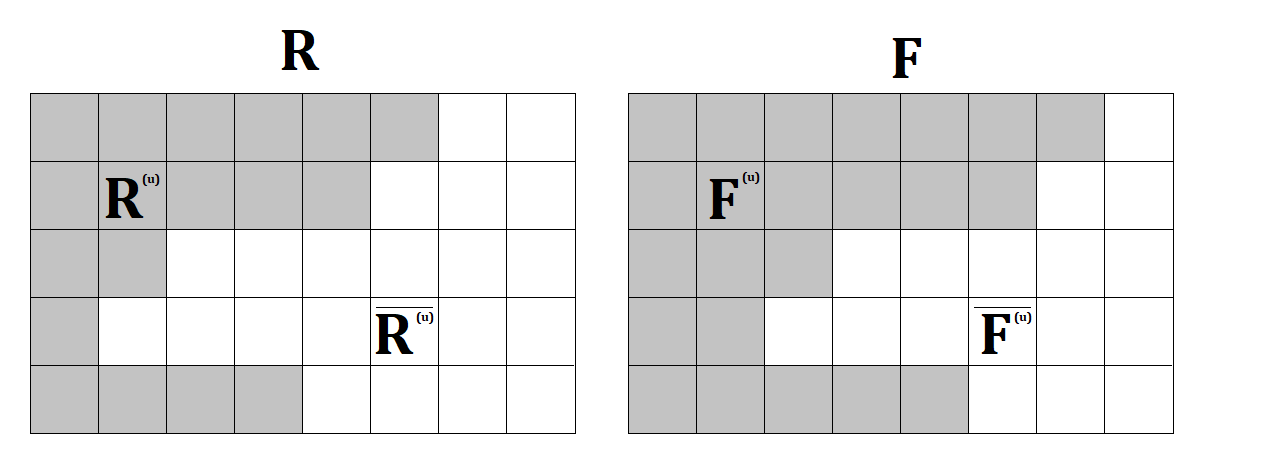
\includegraphics[width=\linewidth]{R grid.png}
	\end{figure}
	\newpage
	The protocol proceeds as follows: 
	\begin{enumerate}
	\item The prover sends \textbf{R}, and \textbf{F} which they calculate using their unlimited computing power. \item Using the classical verification protocol described in \hyperref[she92]{[She92]} for each pair of rows in the above table (\textbf{R}$_i$,\textbf{F}$_i$), the verifier rejects the proof if any pair contain an invalid proof that the input formula evaluates to true.
	\item The verifier chooses a vector $u$ uniformly randomly from $\{1,\dots,N\}^m$ and sends it to the prover along with $\overline{\textbf{F}^{(u)}}$.
	\item In the second round, the prover sends $S$ to the verifier, and the verifier calculates \textbf{R}$_{i,j}-$\textbf{S}$_{i,j}$ for each pair $(i,j)$. 
	
	\item The verifier applies $H^{\otimes k}$ to each register of $\overline{\textbf{R}^{(u)}}$ and accepts if and only if $\overline{\textbf{R}^{(u)}}$ contains only zeros.
	\end{enumerate}
	
	The entries in $\textbf{R}$ and $\textbf{F}$ correspond to the random values $r_i$ and functions $f_i$ from the classical protocol. A full proof of correctness is found in \hyperref[wat99]{[Wat99]}, but we provide an outline here. First suppose that a given formula $Q$ is true. We want to show that the verifier accepts it with certainty. The prover also creates an $m\times N$ matrix $R$ of values drawn uniformly randomly from $\mathbb{F}_{2^k}$, where $m,$ $N,$ and $k$ are defined as above. Using the values of $R$, the prover also generates a corresponding $m\times N$ matrix of \textit{correct} polynomials $F$. Each row $F_i$ is formed by defining polynomials $f_{i,j}$ as in the classical protocol, where instead of getting the random values $r_j$ from the verifier, they are taken from the corresponding row $R_i$ of the generated matrix $R$. Thus, $F_{i,j}=f_{i,j}(R_{i,1},\dots,R_{i,N})$, for $i=1,\dots,m,j=1,\dots,N$. The prover then prepares the following state:
		\[\frac{1}{\sqrt{2^{kmN}}}\sum_{i,j}\ket{R_{i,j}}\ket{F_{i,j}}\]
		
		Forming the registers \textbf{R} and \textbf{F} as described in the protocol. Additionally, if the formula $Q$ is correct, the prover sets each $\textbf{S}_{i,j}$ to $\textbf{R}_{i,j}$. The prover then sends this state to the verifier. As we are assuming $Q$ is true, the honest verifier will not reject at this point, and they will return $\overline{\textbf{F}^{(u)}}$ and $u$ to the prover in response. Then, for each $(i,j)$ define a unitary:
		\[U_{i,j}:\ket{R}\ket{0}\mapsto\ket{R}\ket{F_{i,j}}\]
		The prover then applies $U_{i,j}^{-1}$ to registers $\textbf{S}_{i,j}$ and $\textbf{F}_{i,j}$ for all $\textbf{F}_{i,j}$ in $\overline{\textbf{F}^{(u)}}$, which keeps $\textbf{S}$ the same, but returns all of $\overline{\textbf{F}^{(u)}}$ to $\ket{0}$. After the verifier subtracts each \textbf{R}$_{i,j}$ from each \textbf{S}$_{i,j}$, the registers in $\overline{\textbf{R}^{(u)}}$ will no longer be entangled with any other registers; therefore each register in $\overline{\textbf{R}^{(u)}}$ is sent to $\ket{0}$, and the verifier will accept $Q$ with certainty.\\
		
		Not discussed in this paper, but available in \hyperref[wat99]{[Wat99]}, is the case where $Q$ is not a true formula. In this case, it turns out that the verifier can be made to accept only with some small error probability. An upper bound for this probability is determined by $m$ and $k$. If we choose $m=(d+1)N$ and $k=2d+6+\lceil\log(dm)\rceil$, then $\varepsilon<2^{-d}$, i.e. the error probability is exponentially small in the length of $Q$.
	\end{proof}
	
	\noindent Therefore, we can show that \textbf{PSPACE} $\subseteq$ \textbf{QIP[2]}; moreover, there is an $\varepsilon<2^{-|x|}$ $2$-round quantum protocol for any language $L$ in \textbf{PSPACE}.  
	\subsection{QMA}
	Having now introduced quantum interactive proof systems and the classical class \textbf{MA}, we can discuss its natural extension \textbf{QMA}.
	\begin{defn}
		A language $L$ is in said to be in the class \underline{\textbf{QMA}} if there exists a family of polynomial-time quantum circuits such that:
		\begin{enumerate}
			\item If $x\in L$, then there exists a state $\ket{\Psi}$ such that $P(\text{Circuit accepts } \ket{\Psi})>\frac{2}{3}$
			\item If $x\notin L$, then for any state $\ket{\Psi}$, $P(\text{Circuit accepts } \ket{\Psi})<\frac{1}{3}$
		\end{enumerate}
	\end{defn}
	 There are several important results to do with this class. For example, it has been shown by Kitaev that \textbf{QMA} $\subseteq$ \textbf{P$^{\sharp P}$} (\hyperref[kit99]{[Kit99]}). Another result of Marriott and Watrous is that \textbf{QMA} $\subseteq$ \textbf{PP} (\hyperref[mar05]{[Mar05]}), and further, if the reverse containment holds, i.e. if \textbf{QMA} = \textbf{PP}, it can be shown that \textbf{PH} $\subseteq$ \textbf{PP} (\hyperref[vya03]{[Vya03]}).
    \section{Group Theoretic Applications}
    Having introduced it in the previous section, we proceed to discuss \textbf{QMA} in the context of group theory. The principal result of \hyperref[wat00]{[Wat00]} is a proof of the fact that the group non-membership problem is in \textbf{QMA}. This section will review the proof of this fact, along with some corollaries that allow us to recover various other group properties. 
    \subsection{Group Non-Membership}
    We start by defining the group non-membership problem (GNM).
    \begin{defn}
    	Given a finite group $G$ and $k+1$ elements $g_1,g_2,\dots,g_k,h\in G$, the group non-membership problem asks whether $h$ is outside the subgroup generated by the elements $g_i$,i.e. is it the case that $h\notin (g_1,\dots,g_k)\subseteq G$?
    \end{defn}
	\begin{rmk}
	It is a result of \hyperref[bab91]{[Bab91]} that there exist oracles with respect to which GNM $\notin$ \textbf{NP} and GNM $\notin\textbf{BPP}$.
	\end{rmk}
	
	This definition makes no mention of any particular representation of the finite group $G$, so the convention used in this paper is to represent group elements as finite length binary strings under some relations. To perform the group operation, we employ a \textit{group oracle} which we denote $B$. 
	\begin{defn}
		A \underline{group oracle} $B$ is a family of bijections $\{B_n\}$, each defined $B_n\colon \{0,1\}^{2n+2}\to  \{0,1\}^{2n+2}$, satisfying certain properties defined below. Given a subset of strings $S\subseteq \{0,1\}^n$, we can define a group on $S$, denoted $G_S(B_n)$ and called a \underline{\textit{black-box group}}, whose operation is given by queries to $B$, as follows:
		\begin{enumerate}
			\item If $x,y\in G_S(B_n)$, we have that $y\cdot x=z$, where $z$ is given by $B_n(0,0,x,y)=(0,0,x,z)$.
			\item If $x,y\in G_S(B_n)$, we have that $y\cdot x^{-1}=z$, where $z$ is given by $B_n(1,0,x,y)=(1,0,x,z)$.
			\item If $x$ or $y\notin G_S(B_n)$, we have that $B_n(c,0,x,y)=(c,1,x,y)$, for $c=0,1$.
		\end{enumerate}
	\end{defn}
	The first and second input bits to the maps $B_n$ are the control and error bits, respectively. The control bit, denoted $c$, controls whether we take the inverse of the second group element in the operation. The error bit, denoted $b$, is initialized to $\ket{0}$, and is flipped to $\ket{1}$ exactly when at least one input bit is not a group element. It should be noted that any finite group can be interpreted as a black-box group under some oracle, supposing that we encode its elements as binary strings in a suitable way.\\
	
	Given that each map in $B$ is defined as a bijection, and is hence invertible, we can take each $B_n$ as a definition for a quantum gate acting on $2n+2$ qubits written in the usual computational basis.
	\begin{thm}
		The Group Non-Membership Problem is in \textbf{QMA$^B$} for an arbitrary group oracle $B$.
	\end{thm}
	\begin{proof}
		Let $G$ be a finite group whose elements are written as binary strings of length $n$, let $h\in G$ be a distinguished element, and suppose for some $g_1,\dots,g_k\in G$, we have $H=(g_1,\dots,g_k)\subseteq G$ a finitely generated subgroup of $G$. We aim to determine whether $h\in H$. To this end we define a quantum circuit as follows:\\
		
		 For any subset $A\subseteq G$, we define the state $\ket{A}:=|A|^{-1/2}\sum_{g\in A}\ket{g}$. Let \textbf{R} be an input register initialized to the state $\ket{H}$, and \textbf{B} be an input qubit initialized to $\ket{+}$. Taking the state $\ket{+}\ket{H}$, we multiply by $h$ by applying a controlled $B_n$ gate, whose output will be:
		 \[\frac{1}{\sqrt{2}}\ket{0}\ket{H}+\frac{|H|^{-1/2}}{\sqrt{2}}\sum_{g\in H}\ket{1}B_n(0,0,g,h)=\frac{1}{\sqrt{2}}\ket{0}\ket{H}+\frac{1}{\sqrt{2}}\ket{1}\ket{Hh}\]
		 Then apply a Hadamard gate to the first register, taking us to:
		 \[\frac{1}{2}(\ket{0}(\ket{H}+\ket{Hh})+\ket{1}(\ket{H}-\ket{Hh}))\]
		
		If $h\in H$, then $H=Hh$, so $\ket{H}-\ket{Hh}=0\cdot\ket{H}$, so if we measure \textbf{B} in the $Z$-basis, we will measure $\ket{0}$ with certainty. If $h\notin H$, then the probability that we measure $\ket{1}$ is $\frac{1}{2}$, as $H$ and $Hh$ are disjoint cosets of $G$. Thus, if we can create $m$ copies of the state $H$, a verifier can tell with certainty that $h\in H$ whenever it's true, and will be deceived by the prover with probability $\frac{1}{2^m}$ when $h\notin H$.\\
		
		Therefore, we have shown that, in the case where $h\not H$, if the prover sends polynomial many copies $\ket{H}$ as a certificate, then the verfier will accept the true statement that $h\notin H$ with near certainty. In particular, the verifier will accept with probability higher than the requisite $\frac{2}{3}$ bound for \textbf{QMA}. Additionally, the verifier will reject false claims that $h\notin H$ with certainty, also meeting the \textbf{QMA} requirement. \\
		
		A major caveat for this conclusion is that, in the event that $h\in H$, the dishonest prover need not send $\ket{H}$, and may opt to send any arbitrary $\ket{\Psi}$ instead (to deceive the verifier). The remedy involves making use of the additional power available to the verifier in \textbf{QMA} to first perform a verification that the received certificate $\ket{\Psi}$ is equal to $\ket{H}$. The discussion and completion of proof after this consideration is fully detailed in \hyperref[wat00]{[Wat00]}, making use of a lemma of \hyperref[bab85]{[Bab85]}, but the conclusion is that despite the potential roadblocks presented by the prover's behaviour, we can still recover a QMA protocol that operates with exponentially small error.
	\end{proof}
	An important result (not proved in this paper) is that there is a strict advantage in moving from \textbf{MA} to \textbf{QMA} in that, there exists an oracle $B$ relative to which GNM $\notin$\textbf{MA$^B$}. This separation in the GNM problem additionally leads to the complexity theoretic result that there exists some oracle $B$ such that \textbf{BQP$^B$} $\not\subseteq$ \textbf{MA$^B$} (\hyperref[wat00]{[Wat00]}).  
    \subsection{Other Applications}
    We conclude this section by considering some important corollaries of the main result of the previous section. The fact that we can provide succinct (polynomial sized) proofs of group non-membership in the context of \textbf{QMA} allows us to also produce results in the same context for problems involving several other group-theoretical properties, including:
    \begin{enumerate}
    	\item The \textbf{Proper Subgroup} problem: given a group $G$ and elements $g_1,\dots,g_k,h_1,\dots,h_l\in G$, is it the case that $(h_1,\dots,h_l)\subsetneq (g_1,\dots,g_k)$?
    	\item The \textbf{Divisor of Order} problem: given a group $G$ and an integer $N$, do we have that $N$ divides $|G|$?
    	\item The \textbf{Subgroup Simplicity} problem: given a group $G$ and a subgroup $H=(g_1,\dots,g_k)\subseteq G$, is $H$ simple (no non-trivial normal subgroups)?
    	\item  The \textbf{Maximal Normal Subgroup} problem: given a group $G$ and elements $g_1,\dots,g_k,h_1,\dots,h_l\in G$, is $(h_1,\dots,h_l)$ a maximal normal subgroup of $(g_1,\dots,g_k)$? 
    \end{enumerate}
	It turns out that as corollaries of GNM$\in$\textbf{QMA$^B$}, problems $1$ and $2$ are also both in \textbf{QMA$^B$} for some oracle $B$, while problems $3$ and $4$ are actually in \textbf{co-QMA$^B$}  (\hyperref[bab92]{[Bab92]}).
	
	\section{Conclusion}
	This paper introduced quantum interactive proof systems by discussing primarily two results of Watrous. The first result is that any language in \textbf{PSPACE}, a language which can be solved with a polynomial-sized memory can be equivalently determined using only two rounds of communication between  prover and verfier with access to quantum computations. This result was established incrementally over time by Watrous, who originally showed that such languages belonged to \textbf{QIP[k]}, for some constant $k$-round quantum interactive proof systems. This result was then tightened to $k=3$, then finally $2$. It is possible that this result could be even further tightened to the $1$-round case, or to the $0$-round case (wherein the verifier can simply solve the problem themselves). It is still open as to what languages are characterized by \textbf{{QIP[k]}} for $k>2$. We could also establish relationships between \textbf{PSPACE} and other classes by asking whether they have quantum proof systems, for example we can ask about the relationship between \textbf{NEXP} and \textbf{QIP}.\\
	
	The second portion of this paper was dedicated to the discussion of \textbf{QMA} and its relationship with the group non-membership problem. Some additional group-theoretic applications were discussed at the end of Section 3,  but there are numerous other appplications, e.g. the graph non-isomorphism problem is in \textbf{QMA}. The main direction of continuing research from Section 3 is more so to do with complexity theoretic results related to \textbf{QMA}. Some of these were mentioned in Section 2.1, but one additional direction suggested in \hyperref[wat00]{[Wat00]} is to ask whether \textbf{co-NP} $\subseteq$ \textbf{QMA}, and if so whether there are any interesting consequences.
	
	
	\section*{References}
	\begin{tabular}{ l l }
		\label{bab}[Bab85] & L. Babai, Trading Group Theory for Randomness, Proceedings of the Seventeenth\\& Annual ACM
		Symposium on the Theory of Computing, 1985, 421-429.\\
		\label{bab91}[Bab91] & L. Babai. Local expansion of vertex-transitive graphs and random generation in\\ & finite groups. Twenty-Third Annual ACM Symposium on Theory of Computing,\\& 1991, 164-174.\\
		\label{bab92}[Bab92] & L. Babai. Bounded round interactive proofs in finite groups. SIAM Journal on\\& Discrete Math, 1992, 88-111.\\
		\label{gol89}[Gol89] & S. Goldwasser, M. Sipser. Private coins versus public coins in interactive proof \\& systems, Randomness and Computation, volume 5 of Advances in Computing\\& Research, JAI Press, 1989, 73-90.\\
		\label{kit99}[Kit99] & A. Kitaev, Quantum NP, Talk at AQIP’99: Second Workshop on Algorithms in\\& Quantum
		Information Processing, DePaul University, 1999.\\
		\label{kit00}[Kit00] & A. Kitaev, J. Watrous, Parallelization, amplification, and exponential time\\& simulation of quantum interactive proof system,32nd Annual ACM Symposium\\& on Theory of Computing, 2000, 608–617.\\
		\label{mar05}[Mar05] & C. Marriott, J. Watrous, Quantum Arthur-Merlin Games, 2005. \\&https://doi.org/10.48550/arXiv.cs/0506068\\
		\label{she92}[She92] & A. Shen. IP = PSPACE: simplified proof. Journal of the ACM, 1992, 878–880.\\
		\label{vya03}[Vya03] & M. Vyalyi. QMA=PP implies that PP contains PH, 2003\\
		\label{wat99}[Wat99] & J. Watrous, PSPACE has 2-round quantum interactive proof systems, 1999. \\&https://doi.org/10.48550/arXiv.cs/9901015\\
		\label{wat00}[Wat00] & J. Watrous, Succinct quantum proofs for properties of finite groups, 2000. \\&https://doi.org/10.48550/arXiv.cs/0009002\\
		\label{wat09}[Wat09] & J. Watrous, S. Upadhyay, Z. Ji, R. Jain, QIP=PSPACE, 2009.
		\\&https://doi.org/10.48550/arXiv.0907.4737
		
	\end{tabular}
	
		
\end{document}